\section*{Methodology}
After having converted networks into vectors in the feature space, there are a number of possible ways to analyze the distribution of points and labels and possibly learn the concept that governs such distribution in the feature space. In this study, we use random forest classifier along with the confusion matrix as a way to learn the underlying concept that differentiates different classes of networks. As we have seen in the previous section, the distribution of class labels is obviously skewed which leads us to use several sampling methods that are supposed to alleviate the problem. Here, we explain such methodologies in detail.

	\subsection*{Sampling Methods}
Most of the machine learning algorithms perform well on evenly populated instances of multiple classes. However, once this class balance no longer persists, the algorithms perform poorly on minority classes. This problem, called \textit{class imbalance}, causes any machine learning algorithm that is naive to the data set to focus exclusively on the majority class, ignoring any minority classes. One of the most widely used approaches for mitigating the problem is sampling the data set of interest so that the distribution of classes becomes balanced. Although there are many proposed sampling strategies as of now \cite{SurveySampling}, we primarily use three sampling strategies in this study: random over-sampling, random under-sampling and SMOTE \cite{SMOTE}.

 Here we establish the mathematical notations used in explaining sampling methods. Let $S$ be a set of pairs of $\vec{x_i}$ and $y_i$, namely $S =\{(\vec{x_i},y_i)\}$, for $i = 1,...,n$ where $n$ is the number of data, $\vec{x_i} \in X$ is an instance of networks in the $N$-dimensional feature space and $y_i \in Y = \{1,...,C\}$ is a class label associated with the instance $\vec{x_i}$.   


		\subsubsection*{Random Over-sampling}
		Random over-sampling method is one of the simplest strategies for mitigating the class imbalance problem. It over-samples any minority classes to an extent that the number of instances in each class becomes even. Here we explain this sampling method in a mathematical sense. Let $S_{\rm{maj}} \subset S$ be the majority class, meaning a class having the largest number of instances, $S_{\rm{min}}^{j} \subset S$ the $j$th minority class where $j = 1,...,C-1$ and $P$ a set $\{S_{\rm{maj}}, S_{\rm{min}}^{1},...,S_{\rm{min}}^{C-1} \}$ such that
	
	\begin{equation}
	S_{\rm{maj}} \cup S_{\rm{min}}^{1} \cup S_{\rm{min}}^{2},..., \cup S_{\rm{min}}^{C-1} = S,
	\end{equation}
	and
	\begin{equation}
	\forall S_1,S_2 \in P \land S_1 \neq S_2 \Rightarrow S_1 \cap S_2 = \emptyset,
	\end{equation}

	
where $\emptyset$ means an empty set. Let $E_{\rm{min}}^j$ be a set of points that are sampled at uniformly random from a set $S_{\rm{min}}^{j}$ that satisfies the following equality:

	\begin{equation}
	|S_{\rm{min}}| + | E_{\rm{min}}^j | = |S_{\rm{maj}}|.
	\end{equation}
	
 We then append the set $E_{\rm{min}}^j$ to the corresponding set of the minority class $S_{\rm{min}}^{j}$, namely $S_{\rm{min}}^{j} := S_{\rm{min}}^{j} + E_{\rm{min}}^j$. The drawback of random over-sampling is a potential poor generalization due to the overfit of a classifier to the over-sampled instances.
	
	\subsubsection*{Random Under-sampling}
	Random under-sampling, on the other hand, under-samples the majority class, essentially throwing out some data in order to make the ``cloud" of data points sparser. This``throwing out instances" implies an obvious drawback of this sampling method: It discards potentially important instances that compose the backbone of majority classes, implying the true shape of majority class is no longer retained. Here, again, we explain this method using mathematics. Let $S_{\rm{min}} \subset S$ be the minority class, meaning a class having the least number of instances, $S_{\rm{maj}}^{j}$ the $j$th majority class where $j = 1,...,C-1$ and $P$ a set $\{S_{\rm{min}}, S_{\rm{maj}}^{1},...,S_{\rm{maj}}^{C-1} \}$ such that

	\begin{equation}
	S_{\rm{min}} \cup S_{\rm{maj}}^{1} \cup S_{\rm{maj}}^{2},..., \cup S_{\rm{maj}}^{C-1} = S
	\end{equation}
	and
	\begin{equation}
	\forall S_1,S_2 \in P \land S_1 \neq S_2 \Rightarrow S_1 \cap S_2 = \emptyset.
	\end{equation}
	
Let $E_{\rm{maj}}^j$ be a set of points that are sampled at uniformly random from a set $S_{\rm{maj}}^{j}$ that satisfies the following equality:

	\begin{equation}
	|S_{\rm{min}}| = | S_{\rm{maj}}^j -  E_{\rm{maj}}^j |.
	\end{equation}
Then, we subtract the set $S_{\rm{maj}}^j$ by $E_{\rm{maj}}^j$, thus $S_{\rm{maj}}^j := S_{\rm{maj}}^j -  E_{\rm{maj}}^j$.
		
	\subsubsection*{SMOTE}
		\textit{Synthetic Minority Over-sampling Technique}, widely known as SMOTE \cite{SMOTE}, is an alternative sampling method that synthesizes data points in the training set for a classifier. Mathematically speaking, SMOTE is quite similar to random over-sampling, except for how it generates the set $E_{\rm{min}}^j$ for the minority class $S_{\rm{min}}^j$. For each set of the minority class $j$, namely $S_{\rm{min}}^j$, consider $K$ nearest neighbors of a point $\vec{x_i} \in S_{\rm{min}}^j$ in the $N$-dimensional feature space. To generate a new point, first pick up one of the $K$ nearest neighbors, say $\vec{x_{n}}$, then multiply the corresponding feature vector difference with a weight  $\delta$  chosen from an interval $ [0,1]$ at uniformly random and add this vector to $\vec{x_i}$. Therefore, we have a newly synthesized point defined as follows:
		
		\begin{equation}
		\vec{x_{\rm{new}}} = \vec{x_{i}} + \delta*(\vec{x_{n}} - \vec{x_{i}}).
		\end{equation}

And one repeats this procedure for other neighbors of the point $\vec{x_i}$ and construct a set $E_{\rm{min}}^j$. See the figure \ref{smote} for visualization of the synthesizing process.	
		
		\begin{figure}[ht]
		\begin{center}
		\vspace{0.5cm}
		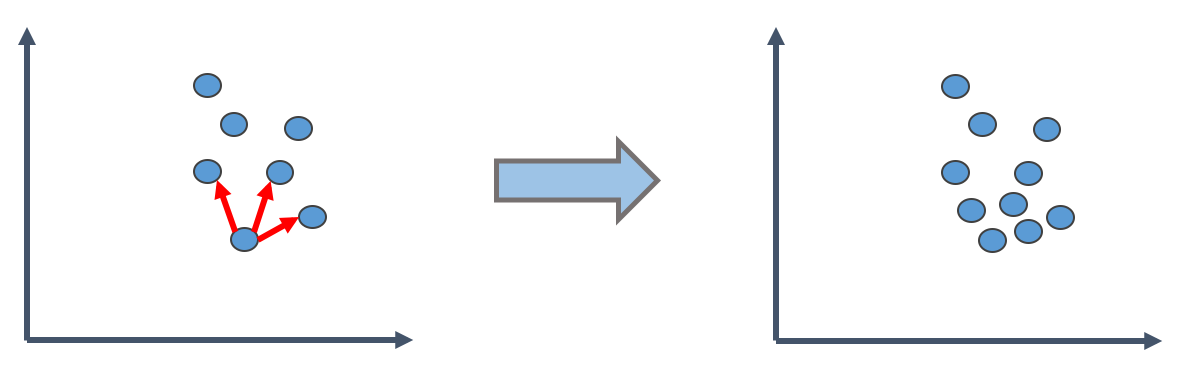
\includegraphics[clip,width=7.5cm,height = 2cm]{figs/SMOTE.png}
		\vspace{0.5cm}
		\caption{Synthesizing phase of SMOTE. Here the number of nearest neighbors $k$ is 3.}
		\label{smote}
		\end{center}
		\end{figure}
		

The core concept of SMOTE is filling out the cloud of minority class instances by interpolating existing data points so that it closely resembles a \textit{convex set}. This idea, making a convex set of minority instances by interpolation, assumes that the shape of a manifold of the underling data distribution itself is convex. In a high dimensional space, it is often the case that the distribution of data forms a quite intricate non-convex manifold on which the data we observe is generated. Therefore one must be careful when using a sampling method like SMOTE that the resulting set of points by interpolation of data points of such complex manifold is likely to be a convex set, that may radically be different from the underlying concept that a classifier tries to learn.

	\subsection*{Classification}
	In order to find similarities and differences of data of different classes, one needs to develop a notion of similarity between the classes. In this study we derive such notion of similarity from confusion matrices that are produced by random forest classifiers. Following sub-sections describe the details of decision tree which is an essential component of random forest, random forest classifier and confusion matrix.
	
		\subsubsection*{Decision Tree}
		Decision tree is a model which describes the relationship between input variables and output class by recursively asking a question on a single input variable and splitting the data set into two based on the answer to the question until a data set has enough homogeneity of a class in it. In a high dimensional space, such spitting the data set corresponds to hyperplane in the space. The algorithm for learning decision tree splits the data set based on a criterion of values of an input variable such that the resulting data sets become less heterogeneous or less``impure" in terms of class labels. One of the widely used such criteria and the one we use in this study is \textit{Gini impurity}. The definition of Gini impurity for a data set with $J$ classes is the following:
	\begin{equation}
		\begin{split}
	I_G(f) = \sum_{i=1}^J f_i(1-f_i) = \sum_{i=1}^J (f_i-f_i^2) \\
	  = \sum_{i=1}^J f_i - \sum_{i=1}^J f_i^2 = 1- \sum_{i=1}^J f_i^2,
		\end{split}
	\end{equation}
where $f_i$ is a probability that an item that belongs to class $i$ is chosen in the data set. Gini impurity becomes $0$ if all items in a set belong to the same class, meaning the set is "pure" and takes a value greater than $0$ if the set contains items of multiple classes. Each splitting essentially seeks the best possible value of an input variable such that the decrease of Gini impurity is the largest when the data set is split at the value (or hyperplane defined with it). Splitting continues until no further improvement can be made and the terminal of a tree are called leaves of the tree, each corresponding to one of the class labels in the data set.
		
	
		\subsubsection*{Random Forest Classifier}
Random forest is a type of \textit{ensemble learning method} that combines a number of so called``sweak" classifiers together \cite{RandomForest}. When it's given a data set to predict after training weak classifiers, it outputs the majority of all outputs from the weak classifiers and this aggregation of weak classifiers prevents random forest from overfitting to the training data. In random forest, such weak classifiers are a decision tree which is explained in the previous section.

The learning phase of random forest classifier first involves random sub-sampling of the original data with replacement for $B$ times, each time the sub-sampled data set is fed to a decision tree. For each decision tree a set of randomly sampled input variables (features) is used for splitting and this random selection of features is called random subspace method or feature bagging. This prevents the classifier to focus too much on feature sets that are highly predictive in the training set. 

One of the advantageous byproducts of random forest is that one can rank input variables or features based on the importance in the classification. Each time a split is made on a node in a decision tree, the decease of Gini impurity can be attributed to selecting a feature as a splitting point.  Calculating the average decrease of Gini impurity for selecting a feature over all decision trees in random forest gives us the importance of the feature that is very consistent with the result of the original method for calculating variable importance \cite{RandomForest,RandomForestOnline}. This ranking of feature importance is the crucial part of the analysis that we describe in the next section.


		\subsubsection*{Confusion Matrix and Similarity}
	A confusion matrix depicts when and how frequently a classifier makes mistakes. The row labels of the matrix usually correspond to  true labels and column labels correspond to predicted labels. An element $c_{ij}$ in a confusion matrix represents the number of occurrences that a classifier predicted an instance of class $i$ as class $j$. So it is easy to notice that diagonal elements of a confusion matrix, namely $c_{ii}$ for $i = 1,...,n$ represents the correct predictions of a classifier. What we are interested in, however, lies in off-diagonal elements of a confusion matrix. The information that a classifier gets confused with classes $i$ and $j$ implies the similarity between classes: if the points of two different classes in a high dimensional feature space are often misclassified as each other, the points of the two classes are in fact close to each other in the feature space, implying that these classes are so similar that a classifier cannot distinguish one from the other. The information in a confusion matrix, when and how frequently a classifier makes mistakes, is essential in order for us to answer one of the questions we have asked: \textit{Are there any sets of network categories that are inherently indistinguishable from each other based solely on network structure?}

It is tempting to use a confusion matrix as a similarity matrix owing to the fact that off-diagonal elements imply the similarities among class labels. This, using a confusion matrix as a similarity matrix, involves following issues however:
\begin{enumerate}
	\item In a confusion matrix, classes with abundant data tend to have large counts for elements in the matrix due to the abundance of test data whereas classes with fewer data have fewer counts in the matrix.
	\item Usually the confusion matrix is not symmetrical, but a number of similarity-related methods assume an input matrix has the symmetry.
\end{enumerate}

Therefore we proceed on the following operations in order to derive a similarity matrix based on a confusion matrix:
\begin{enumerate}
	\item Normalize each row $i$ of the confusion matrix so that $\sum_{j=1}^J c_{ij} = 1$
	\item Symmetrize the resulting matrix from operation $1$ by setting each pair of symmetric elements as: $c_{ij},c_{ji} = \max (c_{ij},c_{ji})$
\end{enumerate}
